\chapter{Integración en GNU Radio}\label{ch:gnuradio}
\chapterquote{The radio is playing all the usual, and what's a wonder wall anyway?}{Fran Healy}

\section{Introducción}\label{subc:gr_congen}

Hasta principios de los 2000s, implementar un sistema de RF era una tarea muy costosa debido a la especificidad de los equipos de hardware requeridos y a la necesidad de contar con costosas licencias para el software utilizado en la operación de los mismos. Esto cambió con la aparición de un nuevo paradigma para la construcción de sistemas de RF llamado \emph{Radio Definida por Software} (\emph{SDR}, por sus siglas en inglés). SDR es un sistema de RF donde la mayor cantidad de elementos están implementados en software.  Este paradigma tuvo un gran crecimiento durante la última década con la aparición de interfaces de RF para computadoras con costos inferiores a los cientos de dólares, como es el caso del dispositivo RTL-SDR, con un costo de alrededor de U\$D 25 \cite{bib:rtl_sdr}, como así también debido al crecimiento de la capacidad de procesamiento de los sistemas informáticos y al crecimiento de la comunidad de software libre dedicada al desarrollo de herramientas de SDR, de la cual salieron aplicaciones de gran utilidad que se utilizan tanto en ambientes educativos y aficionados, como así también en la industria \cite{bib:federico_larocca}. Una de las principales ventajas que tiene SDR sobre las tradicionales implementaciones en hardware dedicado es que permite la actualización y el soporte de múltiples estándares de comunicaciones, siempre y cuando la arquitectura sobre la cual esté instalado este software sea lo suficientemente potente y programable. Esto no es posible en los sistemas tradicionales ya que una actualización o un cambio en una característica requiere el diseño y la implementación de muchos componentes de hardware, tarea costosa y que demanda mucho tiempo \cite{bib:gr_fm}. Otra gran ventaja de los sistemas SDR es que reducen enormemente el tiempo de prototipado, ya que no requiere de la fabricación de hardware específico para probar un diseño.

En la Figura \ref{fig:gr_sdr} se muestra un esquema de un sistema SDR, conformado por una etapa de RF encargada de llevar la señal recibida a banda base o de elevar la señal transmitida a una frecuencia de portadora, una etapa de conversión analógica-digital encargada de obtener las muestras digitales de la señal recibida y de hacer el efecto recíproco en la transmisión, y finalmente una computadora que conforma la arquitectura donde correrá el sistema SDR. En un SDR ideal la etapa de RF se implementa dentro del software, sin embargo esto no es simple de realizar debido a que para lograrlo se debe muestrear la señal de entrada a una frecuencia por encima del doble de la portadora, la cual puede estar por encima de los cientos de megahertz o incluso el gigahertz, solo para obtener información de una señal cuyo ancho de banda es, en general, al menos un orden menor que esta frecuencia. Una alternativa para superar este problema podría ser emplear muestreo pasabanda, pero en general esta solución no suele ser económicamente viable.
% hablar de SDR y basar la intro en base a la primer clase del taller
\begin{figure}[ht!]
    \centering
    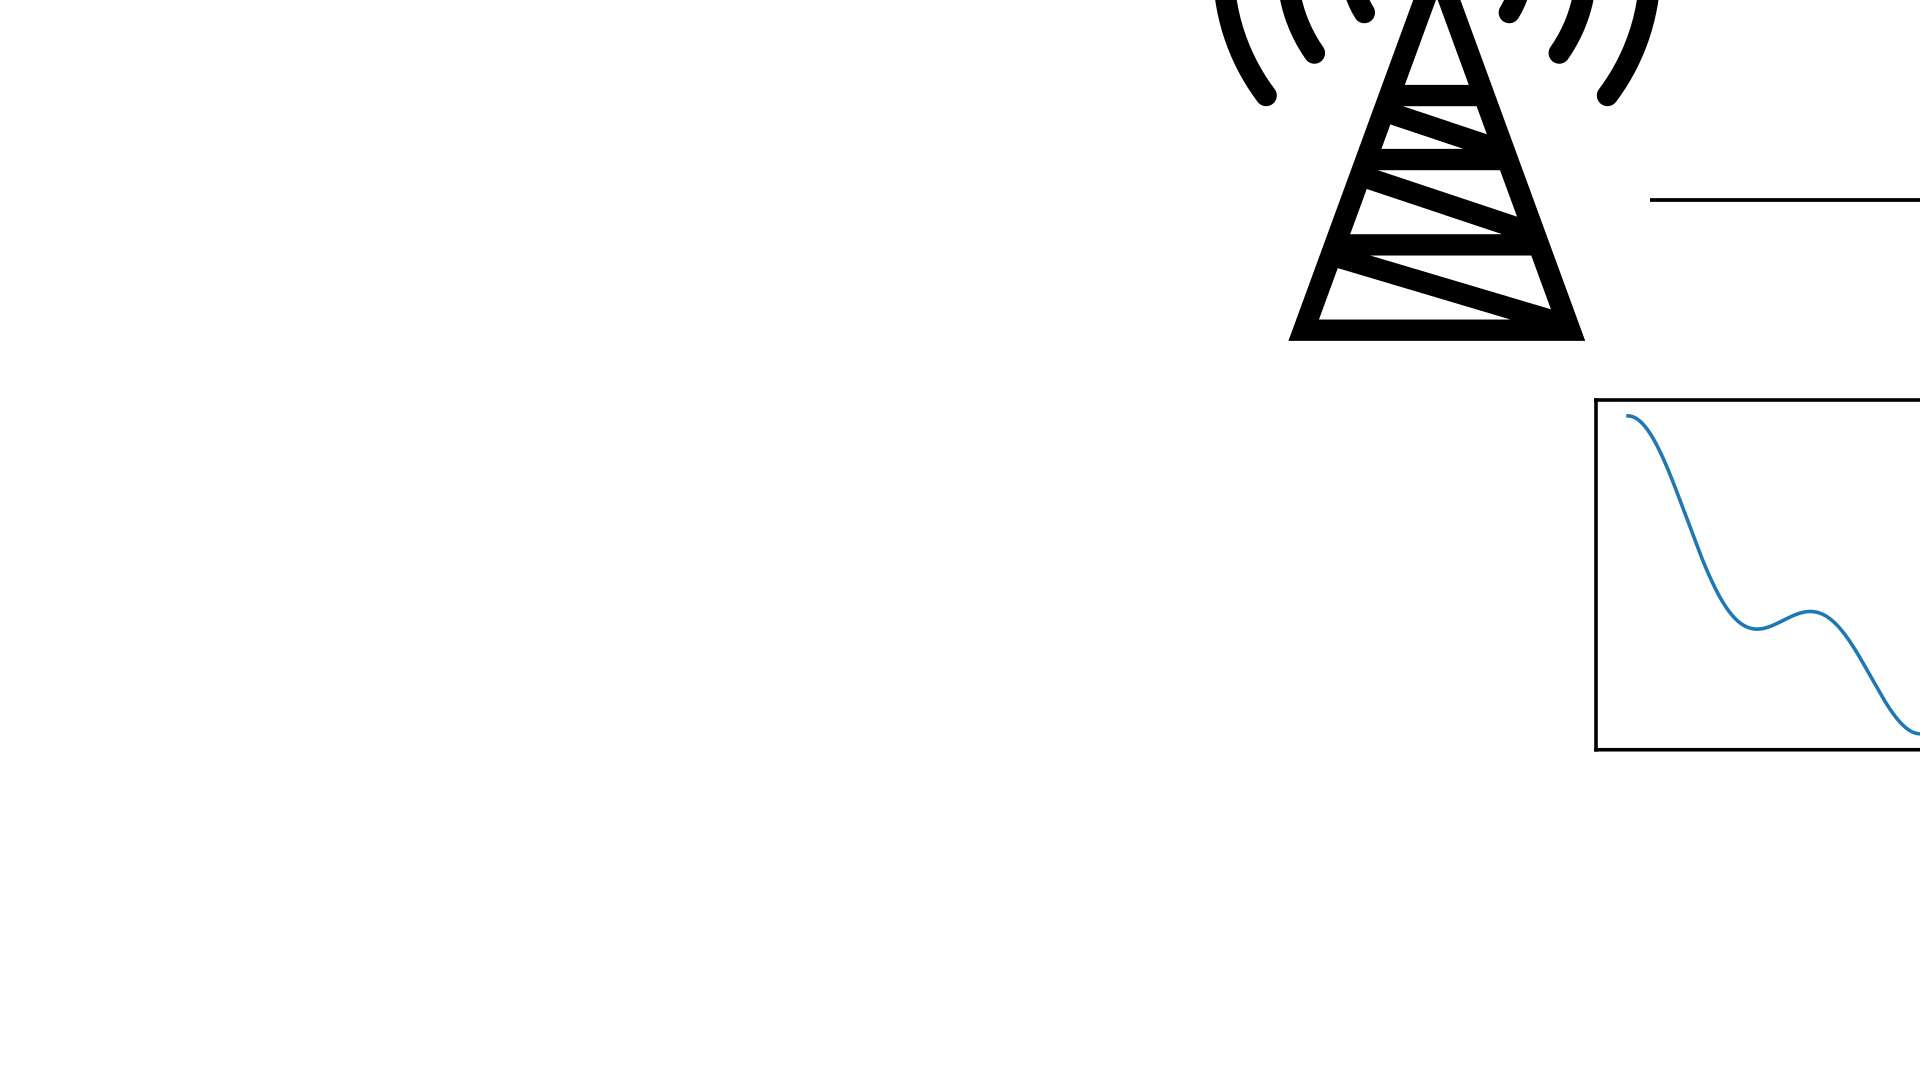
\includegraphics[width=0.9\linewidth]{images/07-GNURadio/gr_sdr.png}
    \caption{Esquema de un sistema de radio definida por software.}
    \label{fig:gr_sdr}
\end{figure}

Dentro del marco de aplicaciones de SDR, \emph{GNU Radio} es el entorno de desarrollo de procesamiento más popular. Esta herramienta provee de bloques de procesamiento de señal que permiten realizar la implementación de sistemas SDR mediante un entorno gráfico llamado \emph{GNU Radio Companion}, el cual es semejante al que proveen herramientas privativas como Simulink\textsuperscript{\textregistered} de la empresa MathWorks\textsuperscript{\textregistered} o LabVIEW\textsuperscript{\texttrademark} de National Instruments\textsuperscript{\texttrademark}. Aparte de permitir la utilización de las librerías de bloques incluidas en la instalación, GNU Radio provee de herramientas e instrucciones para poder generar bloques personalizados mediante programación utilizando los lenguajes \texttt{C++} o \texttt{Python}, como así también permite compartir las librerías creadas entre usuarios. GNU Radio está disponible en los sistemas operativos Microsoft Windows y Linux, sin embargo la versión de Linux es la única que cuenta con soporte oficial. De todas maneras la versión oficial puede ser ejecutada en Windows utilizando el \emph{Windows Subsystem for Linux}, el cual permite ejecutar una instancia de Linux dentro de Windows de una manera más eficiente que ejecutando una máquina virtual.

GNU Radio toma un rol vital en este proyecto, proveyendo no solo la capacidad de realizar la implementación de todo el sistema conformador de haz en software mediante la programación de bloques, sino que, además, entrega un entorno de simulación y prueba de diseños que permite verificar el funcionamiento del sistema en tiempo real.

\section{El modelo equivalente banda base}
Debido a que, como se dijo, al trabajar en SDR las señales deben ser llevadas a banda base para disminuir la frecuencia de muestreo requerida en el software, las muestras con las que se trabaja son de tipo complejo, algo que en principio puede resultar poco intuitivo para el usuario. Para demostrar la relación entre estas muestras complejas y las señales originales se analiza, primero, el espectro de señales genéricas de RF montadas sobre una portadora $f_c$. Si se realiza la transmisión de tres señales reales las cuales se montan sobre una portadora $f_c$, con un ancho de banda total $BW<f_c/2$, la magnitud de su espectro es simétrica, como se muestra en la Figura \ref{fig:gr_espectro_fc}, y su espectro de fase es antisimétrico \cite{bib:haykin}.
\begin{figure}[ht!]
    \centering
    \begin{subfigure}[b]{0.9\textwidth}
        \centering
        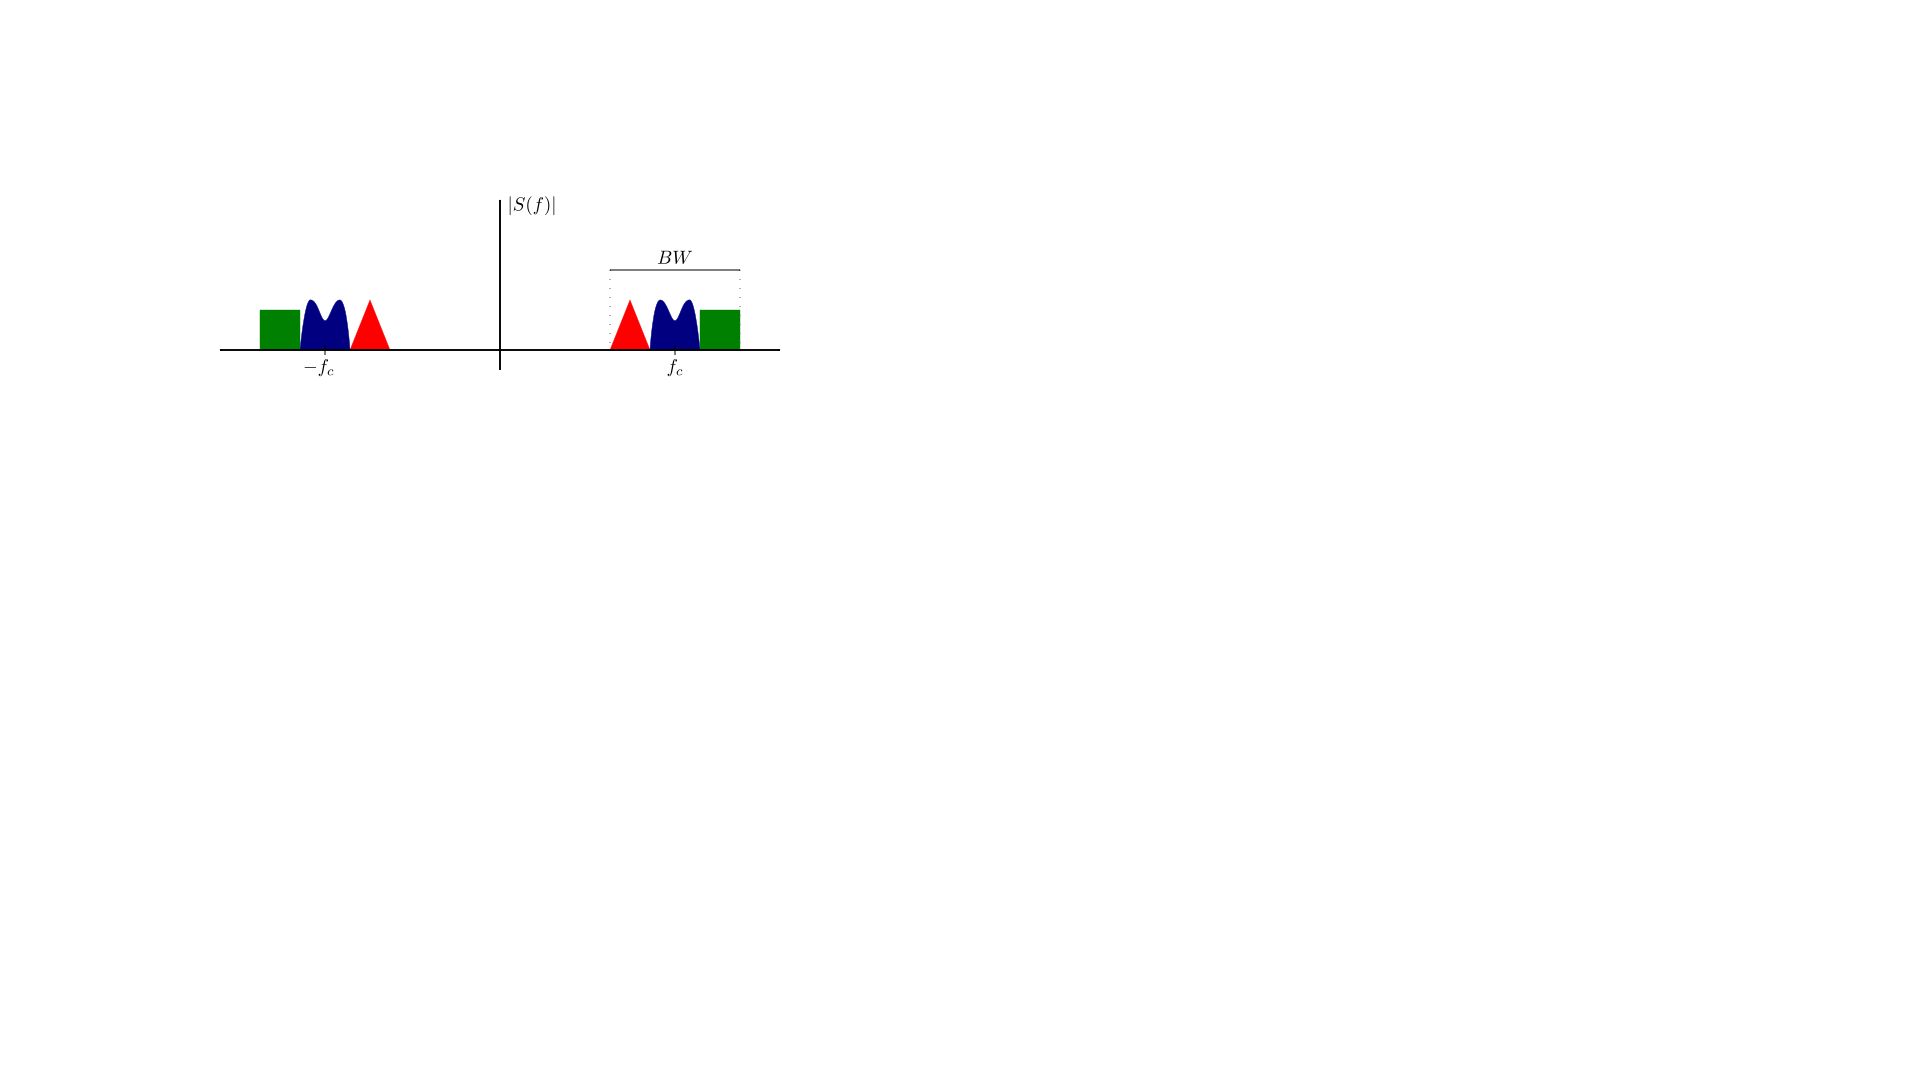
\includegraphics[width=\linewidth]{images/07-GNURadio/gr_espectro_fc.png}
        \caption{Magnitud del espectro de tres señales genéricas montadas sobre una portadora $f_c$.}
        \label{fig:gr_espectro_fc}
    \end{subfigure}
    \hfill
    \begin{subfigure}[b]{0.4\textwidth}
        \centering
        \includegraphics[width=\linewidth]{images/07-GNURadio/gr_espectro_bb.png}
        \caption{Magnitud del espectro en banda base de la señal $S(f)$.}
        \label{fig:gr_espectro_bb}
    \end{subfigure}
    \caption{}
\end{figure}

Si a estas tres señales se las lleva de $f_c$ a banda base se obtiene el espectro de la Figura \ref{fig:gr_espectro_bb}, cuya magnitud no es simétrica, y que, por ende, representa a una señal compleja. El espectro de esta señal en banda base puede escribirse como un corrimiento del espectro de la señal original $S(f)$ haciendo:
\begin{equation}
    S_{bb}(f)=\left\{\begin{matrix}
        \sqrt{2} S(f+f_c) & f+fc>0         \\
        0                 & \textrm{c.o.c}
    \end{matrix}\right.,
\end{equation}
entonces la señal transmitida $S(f)$ puede escribirse a partir de su representación en banda base como \cite{bib:federico_larocca}:
\begin{equation}
    S(f)=\frac{1}{\sqrt{2}}S_{bb}(f-f_c) + \frac{1}{\sqrt{2}}S_{bb}^*(f+f_c)
    \label{eq:gr_sf}
\end{equation}
La representación de $S(f)$ en el dominio temporal puede obtenerse aplicando la antitransformada de Fourier a la Ecuación \ref{eq:gr_sf}, obteniendo la siguiente expresión:
\begin{align}
    s(t) & =\frac{1}{\sqrt{2}} s_{bb}(t) e^{j2\pi f_c t} + \frac{1}{\sqrt{2}}s_{bb}^*(t)  e^{-j2\pi f_c t}   \nonumber \\
         & = \frac{1}{\sqrt{2}} \cdot 2 \cdot \mathrm{Re}\left\{ s_{bb}(t) e^{j2\pi f_c t}\right\}      \nonumber      \\
         & = \sqrt{2} \mathrm{Re}\{s_{bb}(t) \}\cos(2\pi f_c t) - \sqrt{2} \mathrm{Im}\{s_{bb}(t) \}\sin(2\pi f_c t)
    \label{eq:gr_st}
\end{align}
siendo $s_{bb}(t)$ la representación en el dominio temporal de $S_{bb}(f)$. La expresión de la Ecuación \ref{eq:gr_st} muestra la forma de onda en el receptor antes de realizar la conversión a banda base. Si se desea recuperar la señal $s_{bb}(t)$, es decir, la porción del espectro de la señal $s(t)$ que contiene la información de interés, puede multiplicarse la Ecuación \ref{eq:gr_st} por $\sqrt{2}\cos(2\pi f_c t)$ y por $\sqrt{2}\sin(2\pi f_c t)$  obteniendo:
\begin{align}
    s(t)\cdot \sqrt{2} \cos(2\pi f_c t) & = \mathrm{Re}\{s_{bb}(t) \} \underbrace{2 \cos^2(2\pi f_c t)}_{1+\cos(2\pi\cdot 2f_c t)} - \mathrm{Im}\{s_{bb}(t) \}\underbrace{2\sin(2\pi f_c t) \cos(2\pi f_c t)}_{\sin(2\pi\cdot 2f_c t)} \\
    s(t)\cdot \sqrt{2} \sin(2\pi f_c t) & = \mathrm{Re}\{s_{bb}(t) \} \underbrace{2\sin(2\pi f_c t) \cos(2\pi f_c t)}_{\sin(2\pi\cdot 2f_c t)} - \mathrm{Im}\{s_{bb}(t) \}\underbrace{2\sin^2(2\pi f_c t)}_{1-\cos(2\pi\cdot 2f_c t)}
\end{align}
Estas expresiones contienen una componente en banda base de valor $\mathrm{Re}\{s_{bb}(t) \}$ y $\mathrm{Im}\{s_{bb}(t) \}$ sumados a términos centrados espectralmente en $2f_c$, los cuales pueden ser filtrados con un filtro pasa-bajos. A partir de lo obtenido en estas ecuaciones se puede realizar el receptor que se muestra en el diagrama de la Figura \ref{fig:gr_rx} para así obtener las muestras complejas con las cuales se trabaja en SDR.

\begin{figure}[ht!]
    \centering
    
\includegraphics[width=0.9\linewidth]{images/07-GNURadio/gr_rx.png}
    \caption{Diagrama de bloques de un receptor de un sistema SDR.}
    \label{fig:gr_rx}
\end{figure}

\section{Implementación de módulos}
A partir de lo diseñado en el Capítulo \ref{ch:sistema} se decidió realizar la implementación de todos los módulos utilizando GNU Radio para realizar simulaciones en tiempo real del sistema completo y, también, para dejar implementados los subsistemas que posteriormente se instalarán en el PS de la placa de desarrollo. Como ya se dijo, GNU Radio permite la creación de bloques utilizando los lenguajes de programación \texttt{Python} y \texttt{C++}. La implementación en \texttt{Python} ofrece las ventajas de ser un lenguaje de alto nivel con gran variedad de librerías de uso libre que permiten la implementación de bloques de una manera muy rápida y sencilla comparada con las implementaciones en \texttt{C++}. Sin embargo, al ser un lenguaje intérprete, corre con una gran desventaja en el apartado de rendimiento, ya que las instrucciones de los programas no son ejecutadas directamente por la máquina sino que existe un agente externo, el \emph{intérprete}, que se encarga de leer el código y ejecutarlo. En cambio \texttt{C++}, al ser un lenguaje compilado, los programas son convertidos directamente en instrucciones que el procesador puede interpretar, evitando contar con un intermediario y aumentando la eficiencia en la ejecución \cite{bib:interpretevscompiled}. Es por esto que en GNU Radio solo se recomienda implementar bloques en \texttt{Python} en aquellos casos en donde las funciones que realizan no son críticas en el desempeño del sistema, o en aquellos casos en los que se requiere hacer prototipado de bloques para pruebas de funcionamiento rápidas \cite{bib:federico_larocca}.
%Diferencias entre python y c++: 
En esta sección se mencionan algunas características de GNU Radio que se utilizaron para la implementación de los bloques necesarios.

\subsection{Tipos de datos en GNU Radio}
Las interfaces de los bloques en GNU Radio deben tener asignados un tipo de datos definido, los cuales cada uno tiene asignado un color específico. Los tipos de datos permitidos en GNU Radio juntos con su código de color se muestran en la Figura \ref{fig:gr_datatypes}.
\begin{figure}[ht!]
    \centering
    \includegraphics[width=0.5\linewidth]{images/07-GNURadio/gr_datatypes.png}
    \caption{Tipos de datos disponibles en GNU Radio con su correspondiente identificación de color.}
    \label{fig:gr_datatypes}
\end{figure}

En GNU Radio Companion solo pueden conectarse interfaces de bloques que sean del mismo tipo de datos. Para facilitar esta tarea y evitar errores, las interfaces siguen el código de color definido en la Figura \ref{fig:gr_datatypes}. En la Figura \ref{fig:gr_blockconnection} se muestra un ejemplo de interconexión correcta e incorrecta entre bloques.

\begin{figure}[ht!]
    \centering
    \includegraphics[width=0.6\linewidth]{images/07-GNURadio/gr_blockconnection.png}
    \caption{Conexiones entre bloques. GNU Radio Companion indica con color rojo aquellas conexiones no permitidas.}
    \label{fig:gr_blockconnection}
\end{figure}

GNU Radio permite, además, el uso de tipo de datos \emph{polimórficos}, los cuales son tipos de datos no explícitos que permiten sobrepasar la exigencia del tipado estricto de \texttt{C++} permitiendo declarar un tipo de dato genérico que se define según el contexto de la aplicación. En este proyecto, este tipo de dato es de gran utilidad a la hora de realizar el envío de los ángulos estimados por el subsistema estimador de DOA al subsistema conformador de haz, ya que, a pesar de que estos datos serán siempre reales, el tamaño de los vectores enviados cambiarán según cuántas sean las señales detectadas.

\subsection{Callbacks}
En las simulaciones que se muestran en la Sección \ref{subc:gr_simulaciones} es oportuno contar con la posibilidad de cambiar algunos parámetros en tiempo de ejecución, como por ejemplo variar la DOA de una señal simulada para emular la recepción de un satélite LEO, o variar el piso de ruido de manera tal de poder evaluar en el momento cómo una degradación en la señal afecta la estimación de la DOA. El método que permite realizar esto en GNU Radio se llama \emph{callback}. Los callbacks son funciones que se declaran en cada bloque para cada variable que se desea poder variar en tiempo de ejecución, y son llamadas por GNU Radio Companion en el momento en el que algunas de estas variables se modifica, de manera tal de poder actualizarla en el momento y ver cómo se propaga ese cambio en la simulación.

\subsection{La librería VOLK}

Dentro del proyecto GNU Radio existe un subproyecto llamado \emph{Vector-Optimized Library of Kernels} (\emph{VOLK}), el cual consiste en una librería que contiene kernels de código SIMD\footnote{\emph{Single Instruction, Multiple Data}: técnica de software que permite alcanzar paralelismo a nivel de datos.} para la optimización de operaciones matemáticas orientadas a vectores \cite{bib:volk}. Estas librerías se encargan de analizar y elegir cuáles son las instrucciones del procesador que optimizan la ejecución de las distintas operaciones matemáticas según en qué arquitectura de hardware se está ejecutando el programa. Utilizando estas librerías se puede alcanzar mejoras de rendimiento de hasta un 40\% \cite{bib:federico_larocca}.

\subsection{El emulador de ARU.}

Debido a que en el momento de realización de este proyecto no se cuenta con el arreglo de antenas ni con el sistema de adquisición implementados, la manera de realizar las pruebas de los sistemas desarrollados es emulando el comportamiento de un ARU. Para esto se implementa el bloque que se muestra en la Figura \ref{fig:gr_phasedarray}.

\begin{figure}[ht!]
    \centering
    \includegraphics[width=0.6\linewidth]{images/07-GNURadio/gr_phasedarray.png}
    \caption{Representación como bloque del emulador de ARU para realizar las simulaciones del sistema conformador de haz.}
    \label{fig:gr_phasedarray}
\end{figure}

Este bloque recibe $D$ señales en sus entradas y entrega la matriz de salida $\mathbf{X}$ de tamaño $M\times N$, siendo M la cantidad de elementos del arreglo y $N$ la cantidad de muestras temporales. Para hacer esto se basa en el modelo de datos de la Ecuación \ref{eq:doaest_x} y en la definición del vector de apuntamiento de un ARU definido en la Ecuación \ref{eq:beamforming_a_aru}. Este bloque debe ser configurado con la cantidad de elementos del arreglo en ambas direcciones, identificados por $M_x$ y $M_y$, las direcciones de arribo de las $D$ señales emuladas, identificadas con los símbolos $\bar{\theta}$ y $\bar{\varphi}$, las frecuencias de portadoras de las señales recibidas $\bar{f_c}$, la distancia de separación entre elementos del arreglo $d$ y el error en esta distancia $\frac{\sigma_d}{d}$.

\section{Simulaciones}\label{subc:gr_simulaciones}

A partir de lo analizado se implementaron los cuatro bloques necesarios para realizar la simulación del sistema completo, estos son:
\begin{itemize}
    \item \textbf{Phased Array Emulator:} emulador de un ARU programado en \texttt{C++} utilizando VOLK que recibe muestras de señales complejas y entrega el vector de muestras complejas $\bar{x}$ emulando las salidas de cada elemento de un ARU.
    \item \textbf{Random Sampler:} muestrador aleatorio como se mostró en la Sección \ref{subc:sistema_randomsampler}, programado en \texttt{C++}, el cual entrega a la salida los vectores de entrada muestreados aleatoriamente.
    \item \textbf{DOA ESPRIT Estimation:} bloque programado en \texttt{Python} que ejecuta el algoritmo de estimación de DOA ESPRIT, recibiendo vectores de muestras complejas provenientes del muestreador aleatorio y entregando un mensaje polimórfico que contiene vectores reales correspondientes cuyos elementos corresponden a los ángulos de elevación y azimut de las señales detectadas.
    \item \textbf{Beamformer:} bloque programado en \texttt{C++} usando VOLK que recibe vectores de muestras complejas y los ángulos de arribo detectados por el bloque DOA ESPRIT Estimation en forma de mensaje polimórfico y entrega a su salida las muestras de las señales conformadas.
\end{itemize}

En la Figura \ref{fig:gr_sim0_companion} se muestra una captura del diagrama de bloques de la simulación de una transmisión QPSK utilizando el sistema completo en GNU Radio Companion. En la Figura \ref{fig:gr_sim0_qt} se muestra la constelación de la señal entregada por el conformador de haz, la cual corresponde a la señal QPSK transmitida.

\begin{sidewaysfigure}[t]
    \centering
    \begin{subfigure}[b]{0.9\textwidth}
        \centering
        \includegraphics[width=\linewidth]{images/07-GNURadio/gr_sim0_comp.png}
        \caption{Diagrama de bloques del sistema implementado en GNU Radio. La zona superior del diagrama corresponde a la transmisión y la parte inferior a la recepción.}
        \label{fig:gr_sim0_companion}
    \end{subfigure}
    \hfill
    \begin{subfigure}[b]{0.4\textwidth}
        \centering
        \includegraphics[width=\linewidth]{images/07-GNURadio/gr_sim0_qt.png}
        \caption{Constelación de la salida del sistema conformador de haz al recibir una señal QPSK con una cierta DOA.}
        \label{fig:gr_sim0_qt}
    \end{subfigure}
    \caption{Simulación de transmisión QPSK.}
\end{sidewaysfigure}

Luego de comprobar el correcto funcionamiento del sistema se procede a realizar las pruebas de rendimiento, haciendo hincapié en mediciones de tasa de error de bit (BER) frente a distintos escenarios, y en el procesamiento requerido por cada uno de los subsistemas.

\subsection{El módulo gr-satellites}
El módulo \texttt{gr-satellites} desarrollado por Daniel Estévez \cite{bib:gr-satellites} es uno de los módulos más populares en GNU Radio. Este módulo contiene los bloques necesarios para realizar la recepción y decodificación de señales de una gran parte de los satélites de aficionados existentes. Además cuenta con una gran variedad de ejemplos de simulaciones de transmisiones satelitales que pueden ser utilizadas en este proyecto para brindar un grado más de realismo a las pruebas. En particular en este proyecto se utiliza el ejemplo de medición de tasa de error de bit simulando la recepción de información proveniente del satélite LilacSat-1 \cite{bib:ber-simulation}. Esta simulación realiza esta transmisión utilizando modulación BPSK e iterando para distintos valores de $\frac{E_b}{N_0}$, midiendo la cantidad de errores a la salida y obteniendo una curva de tasa de error de bit. Modificando este ejemplo se agregó el sistema conformador de haz obteniendo el diagrama de bloques que se muestra en la Figura \ref{fig:gr_bersim}.

\begin{sidewaysfigure}[t]
    \centering
    \includegraphics[width=0.9\linewidth]{images/07-GNURadio/gr_bersim.png}
    \caption{Diagrama de bloques utilizado para la medición de tasa de error de bit mediante la simulación de un enlace de comunicación con el satélite LilacSat-1.}
    \label{fig:gr_bersim}
\end{sidewaysfigure}

\subsection{Resultados obtenidos}\label{subc:gr_bertest}

Utilizando el diagrama de la Figura \ref{fig:gr_bersim} se evaluó el desempeño del sistema obteniendo las curvas de tasa de error de bit en función de $\frac{E_b}{N_0}$ para distintos valores de $\frac{\sigma_d}{d}$, obteniendo las curvas que se muestran en la gráfica de la Figura \ref{fig:gr_bersim_resul}.

\begin{sidewaysfigure}[t]
    \centering
    \includegraphics[width=0.9\linewidth]{images/07-GNURadio/gr_bersim_resul.png}
    \caption{Curvas de BER en función de $\frac{E_b}{N_0}$ para distintos valores de errores en la separación de elementos del ARU comparadas con recepción óptima de una transmisión BPSK.}
    \label{fig:gr_bersim_resul}
\end{sidewaysfigure}

Como puede verse, para el caso de ubicación perfecta de los elementos la curva obtenida tiene un desempeño 0,7 dB peor que la recepción óptima de BPSK para una $\textrm{BER}=10^{-6}$. Además, para un error en la ubicación de elementos del 30\%, el desempeño cae 1 dB para este tipo de transmisión.

\subsection{Requerimientos de procesamiento}\label{subc:gr_proc}

Finalmente, se midió el uso del procesador de cada bloque del sistema conformador de haz durante el tiempo de ejecución utilizando la función \texttt{top -H} incluida en Linux, la cual permite ver en tiempo real el consumo de cada proceso que está corriendo en el sistema, obteniéndose los resultados de la Tabla \ref{tab:gr_cpu}\footnote{El hecho de que la suma de los porcentajes sea superior al 100\% se debe a que la simulación está corriendo en una computadora con un procesador de 8 núcleos, y GNU Radio asigna un hilo de ejecución separado para cada bloque para poder ubicar a cada uno en el procesador menos ocupado.}.


\begin{table}[ht!]
    \centering
    \begin{tabular}{|c|c|}
        \hline
        {\color[HTML]{000000} \textbf{Bloque}}       & {\color[HTML]{000000} \textbf{CPU {[}\%{]}}} \\ \hline
        {\color[HTML]{000000} DOA ESPRIT Estimation} & {\color[HTML]{000000} 99,3}                  \\ \hline
        Beamformer                                   & 3,7                                          \\ \hline
        {\color[HTML]{000000} Random Sampler}        & {\color[HTML]{000000} 2,3}                   \\ \hline
        {\color[HTML]{000000} Phased Array Emulator} & {\color[HTML]{000000} 2}                     \\ \hline
    \end{tabular}
    \caption{\label{tab:gr_cpu} Utilización del procesador correspondiente a cada bloque del sistema conformador de haz.}
\end{table}

Como puede observarse, el bloque estimador de DOA con ESPRIT es el bloque que insume la mayor parte de la carga de cómputo en el sistema, principalmente debido a que es el único implementado en \texttt{Python}, por ende, si se desea incrementar la eficiencia para la implementación en la placa de desarrollo, deberá rehacerse en lenguaje \texttt{C++}, utilizando la librería \texttt{Eigen} \cite{bib:eigen} para la implementación de la SVD.